\chapter{Tabele cu rezultate}

\begin{figure}
    \centering
    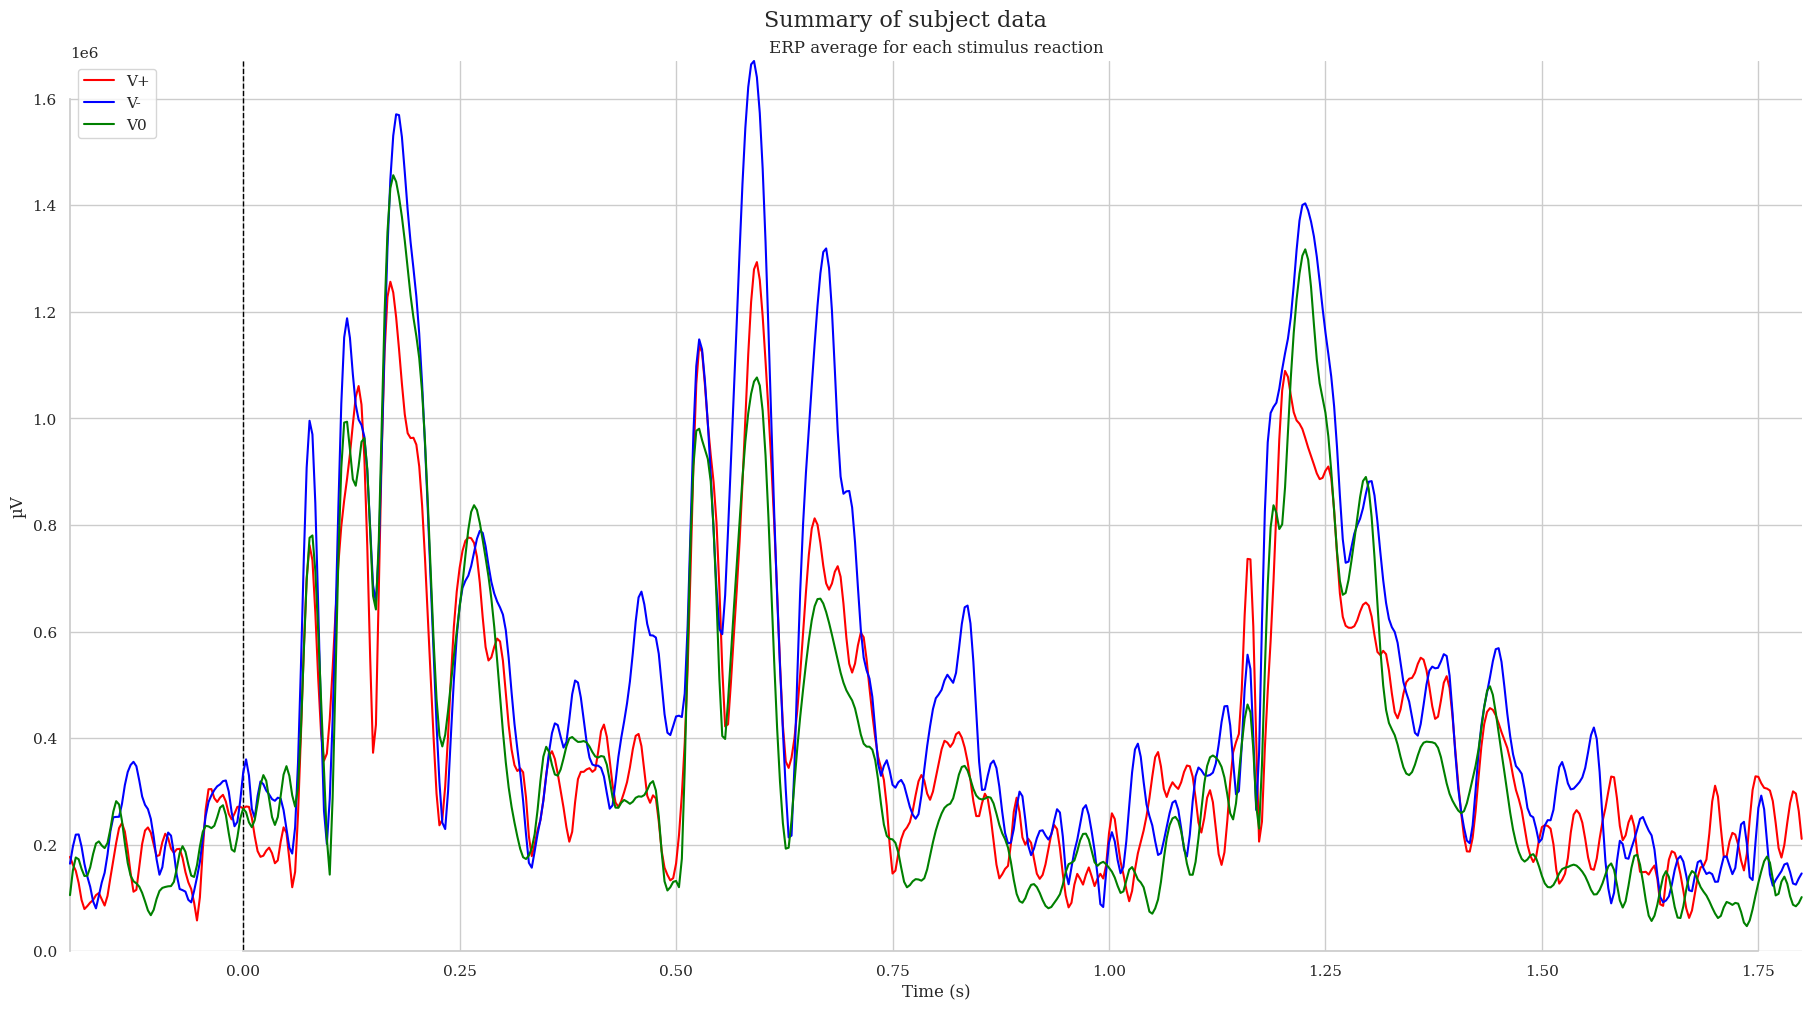
\includegraphics[width=1\linewidth]{images/average_response_each_erp.png}
    \caption{Raspunsul mediu pentru fiecare tip de eveniment}
    \label{fig:average_response_by_event}
\end{figure}

\begin{figure}[h]
    \centering
    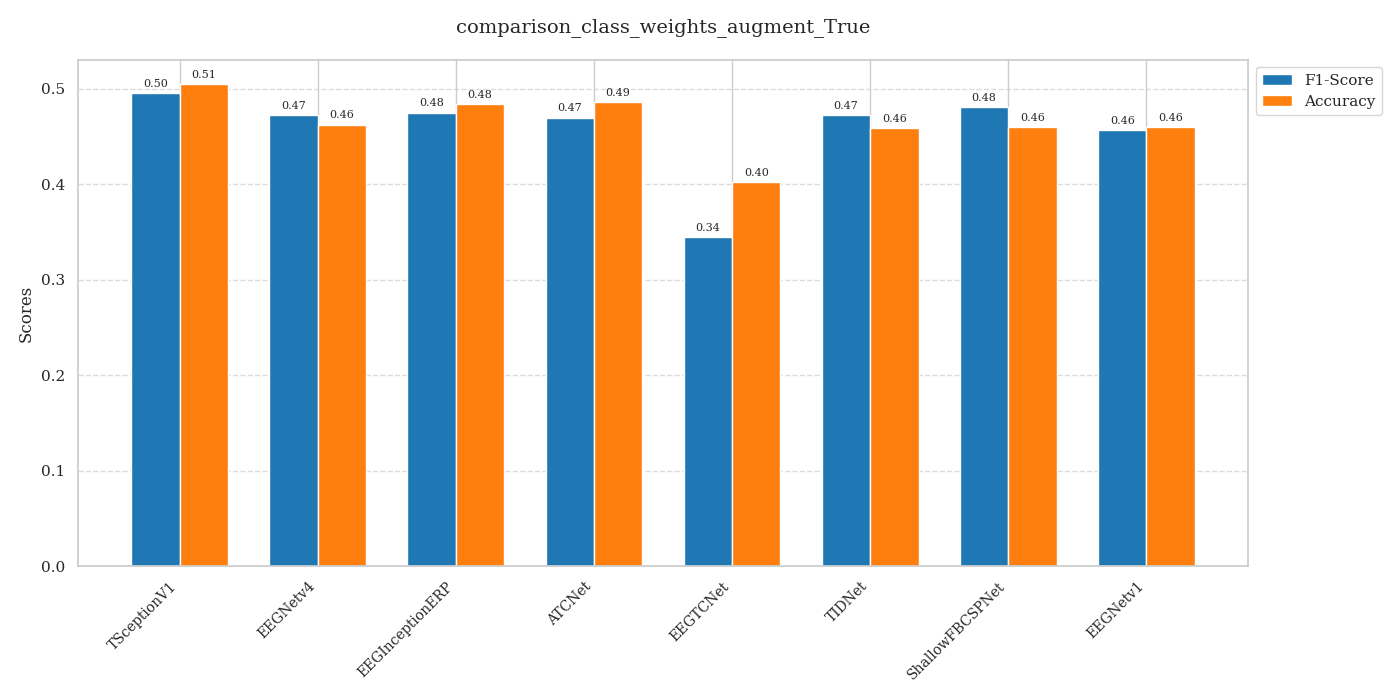
\includegraphics[width=1\linewidth]{images/comparison_class_weights_augment_True.png}
    \caption{Performanta modelelor cu weight-uri de clase si augmentari}
    \label{fig:performance_class_weights_augment_true}
\end{figure}

\begin{figure}
    \centering
    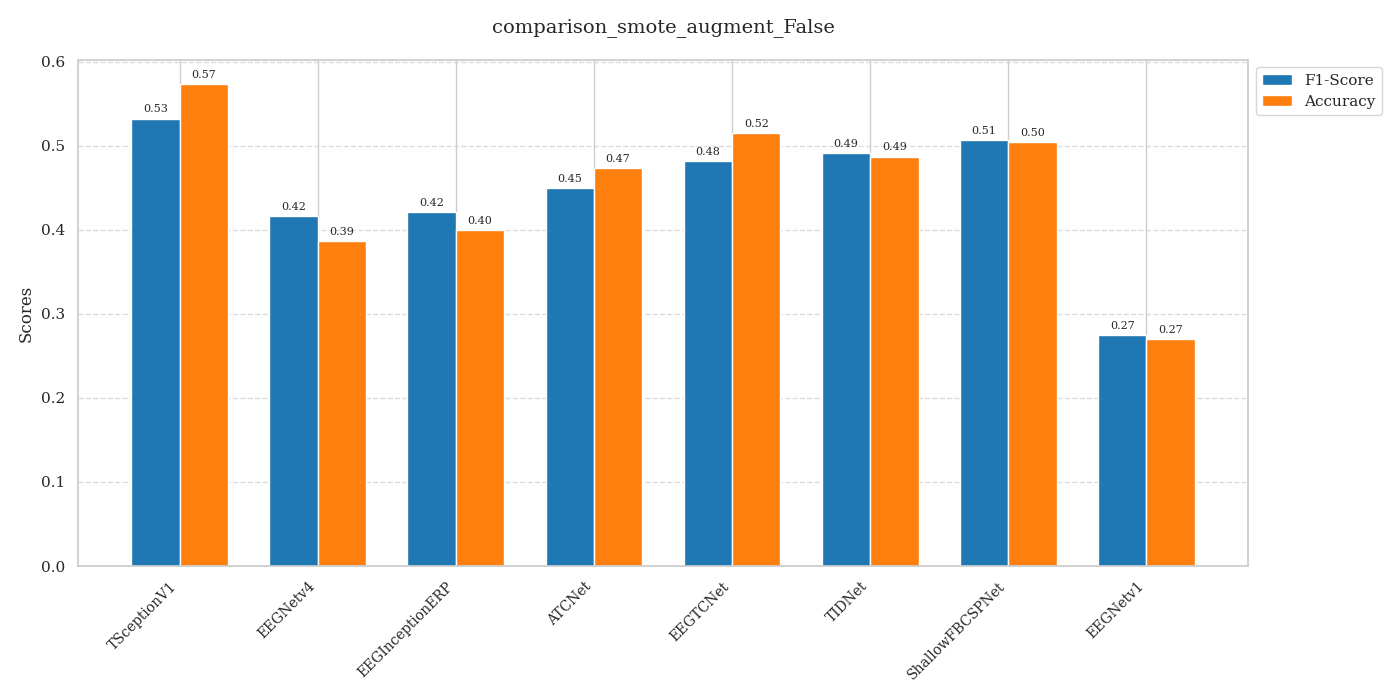
\includegraphics[width=1\linewidth]{images/comparison_smote_augment_False.png}
    \caption{Performanța modelelor folosind date sintetice, fără augmentări}
    \label{fig:smote_augment_false}
\end{figure}

\begin{figure}
    \centering
    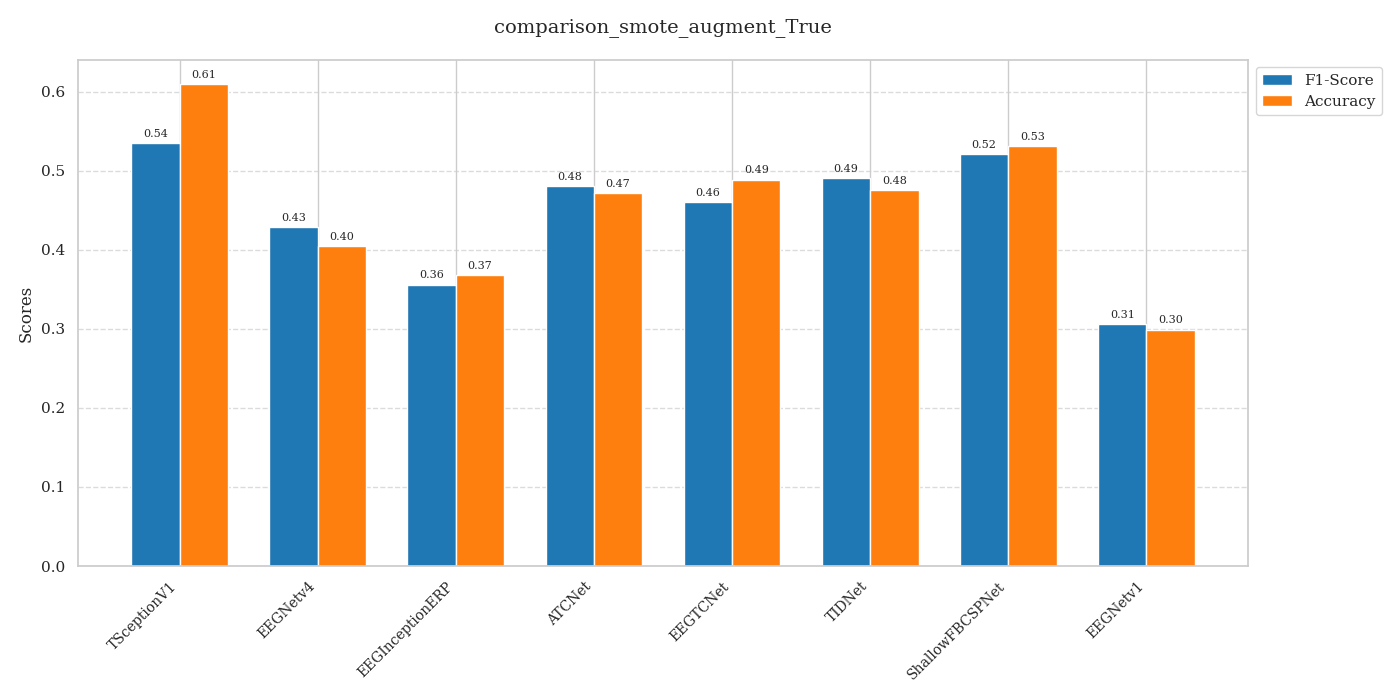
\includegraphics[width=1\linewidth]{comparison_smote_augment_True.png}
    \caption{Performanța modelelor, folosind date sintetice și augmentări}
    \label{fig:smote_augment_true}
\end{figure}

\chapter{Cod sursă}

\begin{figure}[h]
    \centering
    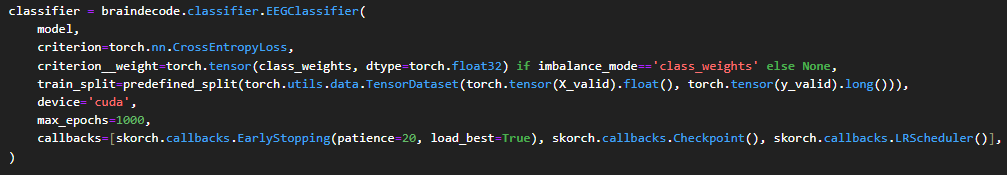
\includegraphics[width=1\linewidth]{wrapper_clasificator_braindecode.png}
    \caption{Apelarea wrapper-ului din braindecode}
    \label{fig:wrapper_braindecode}
\end{figure}

\begin{figure}[h]
    \centering
    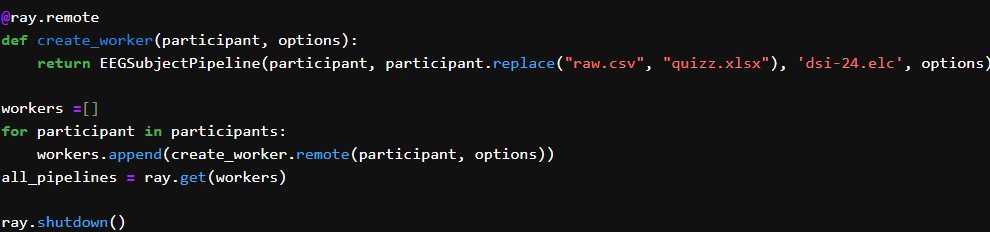
\includegraphics[width=1\linewidth]{images/ray.png}
    \caption{Paralelizare utilizând Ray}
    \label{fig:paralelizare_ray}
\end{figure}

\begin{figure}[h]
    \centering
    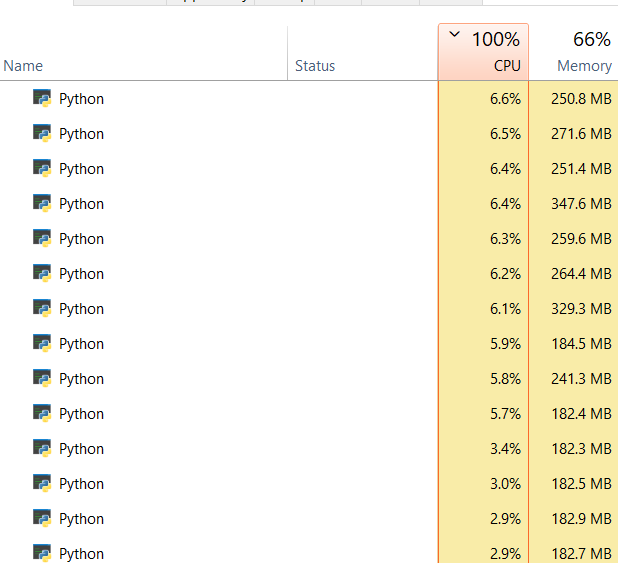
\includegraphics[width=0.7\linewidth]{task_manager.png}
    \caption{Load-ul pe calculator}
    \label{fig:load_calculator}
\end{figure}

\begin{figure}
    \centering
    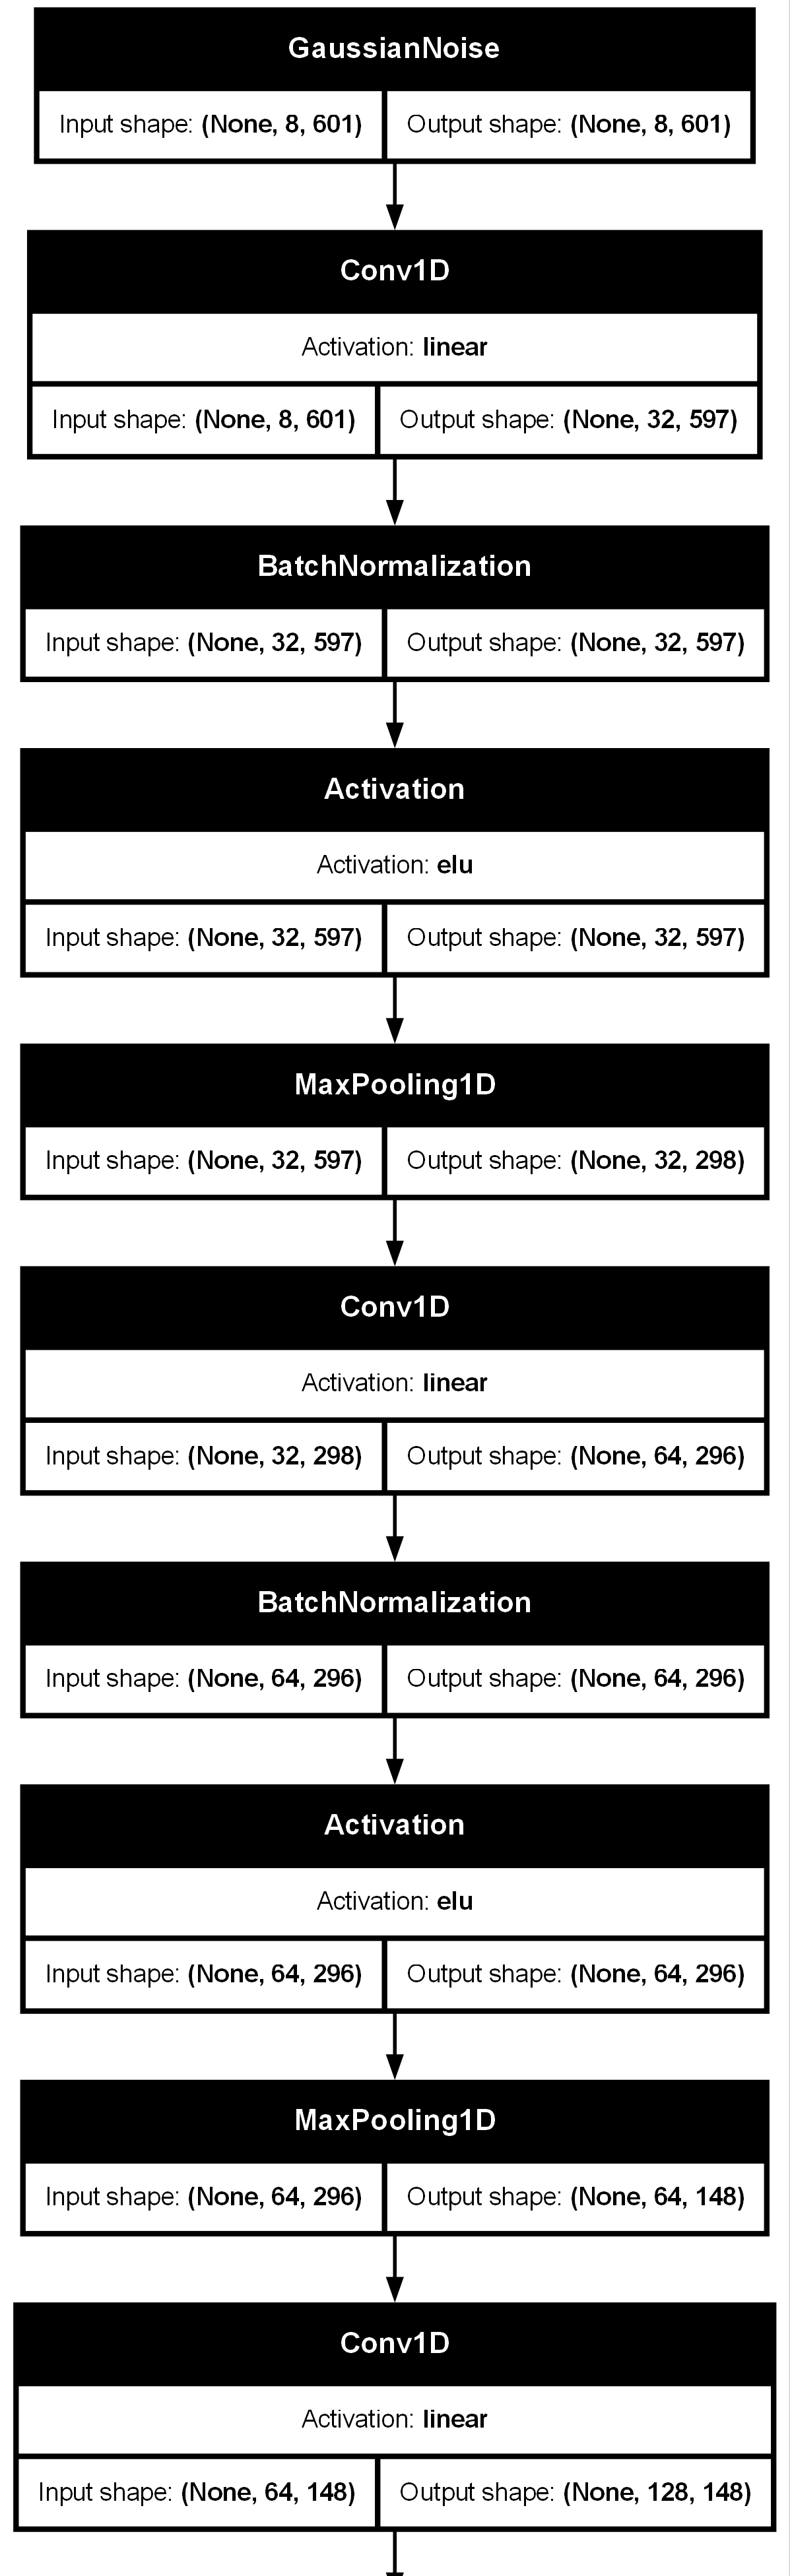
\includegraphics[width=0.4\linewidth]{model_part1.png}
    \caption{Model personal, partea 1}
    \label{fig:model_part1}
\end{figure}

\begin{figure}
    \centering
    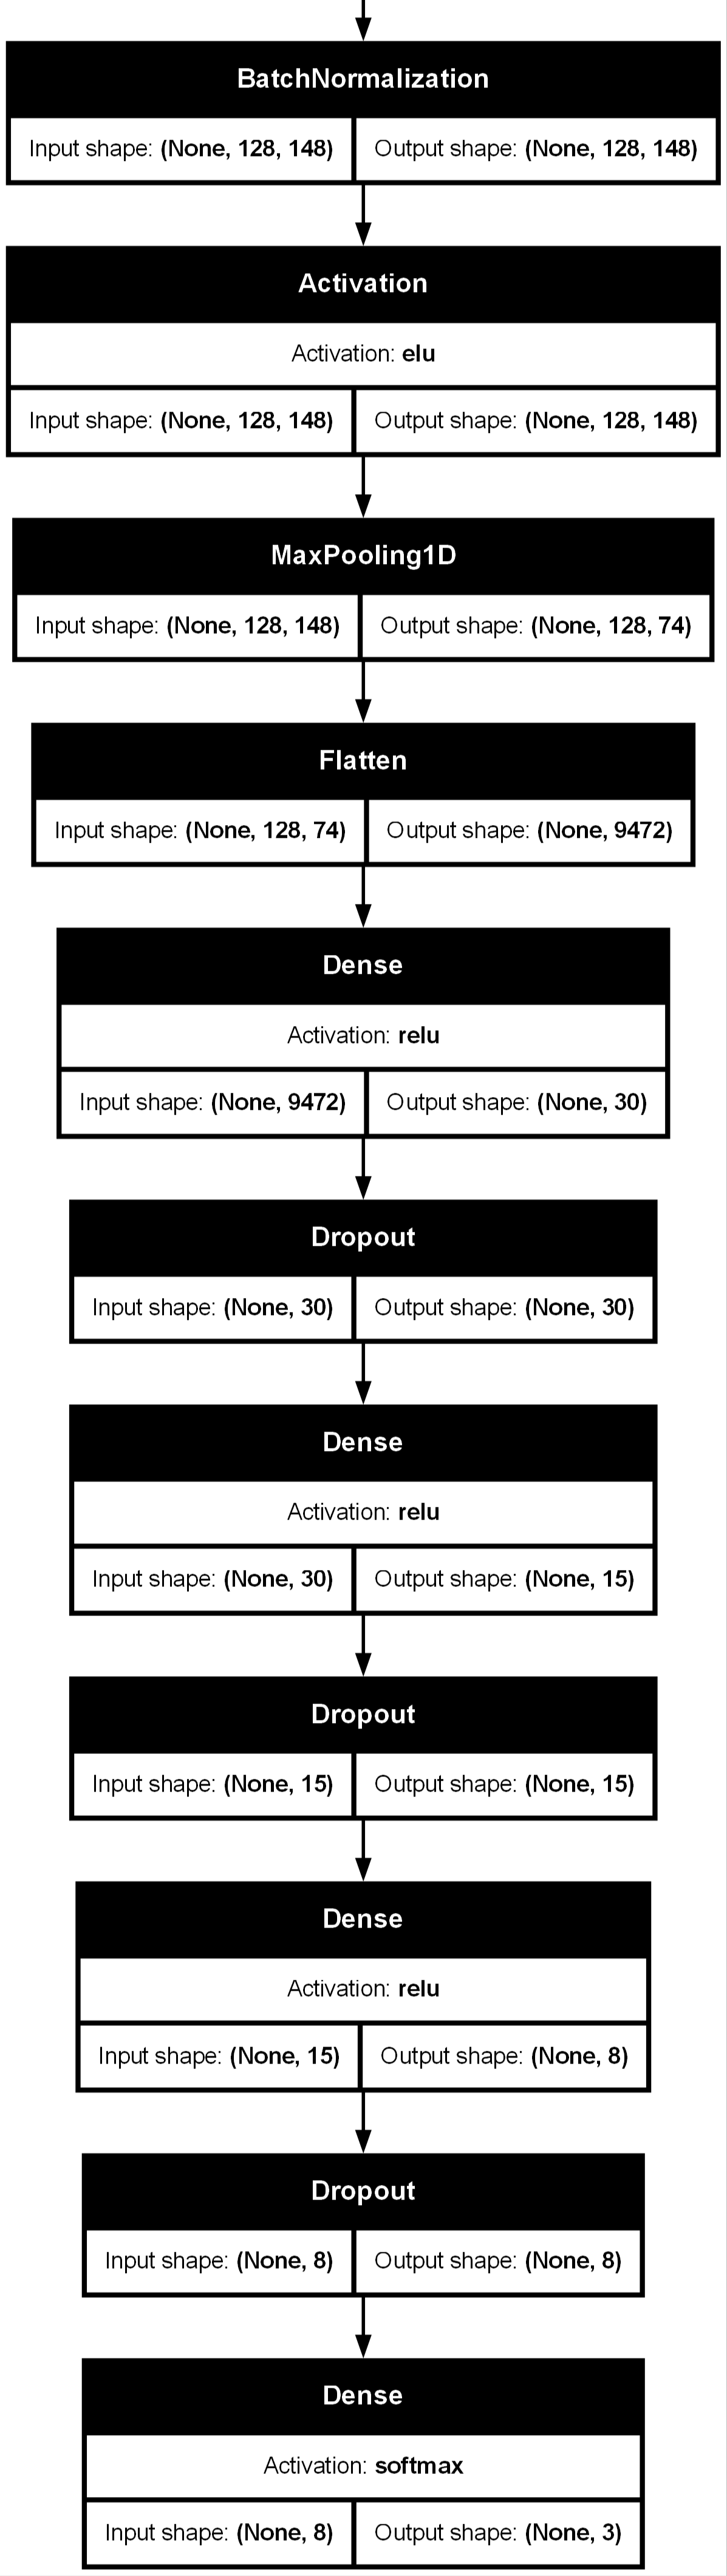
\includegraphics[width=0.4\linewidth]{model_part2.png}
    \caption{Model personal, partea 2}
    \label{fig:model_part2}
\end{figure}

\begin{figure}
    \centering
    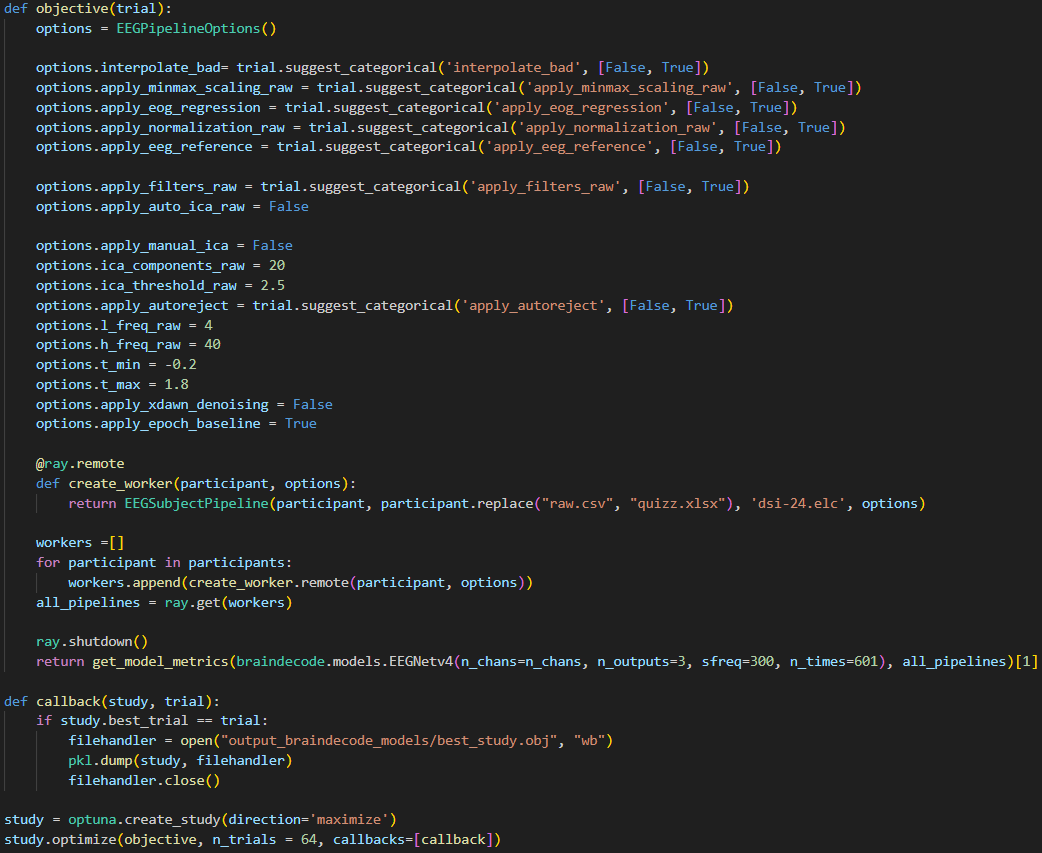
\includegraphics[width=1\linewidth]{optuna_study.png}
    \caption{Cautarea hiperparametrilor folosind optuna}
    \label{fig:optuna_search}
\end{figure}

\begin{figure}
    \centering
    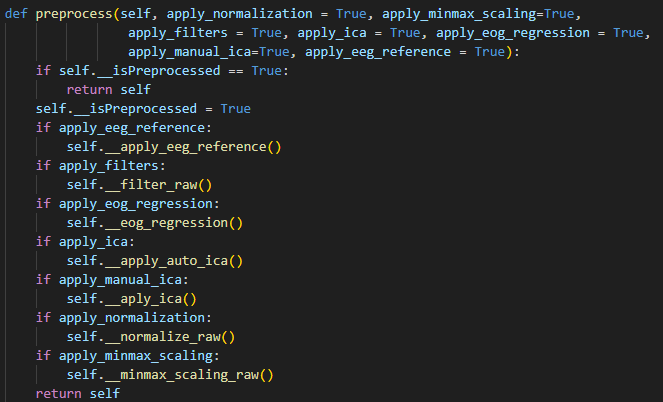
\includegraphics[width=1\linewidth]{images/parametrizare.png}
    \caption{Parametrizarea preprocesării semnalui}
    \label{fig:parametrizare}
\end{figure}

\begin{figure}
    \centering
    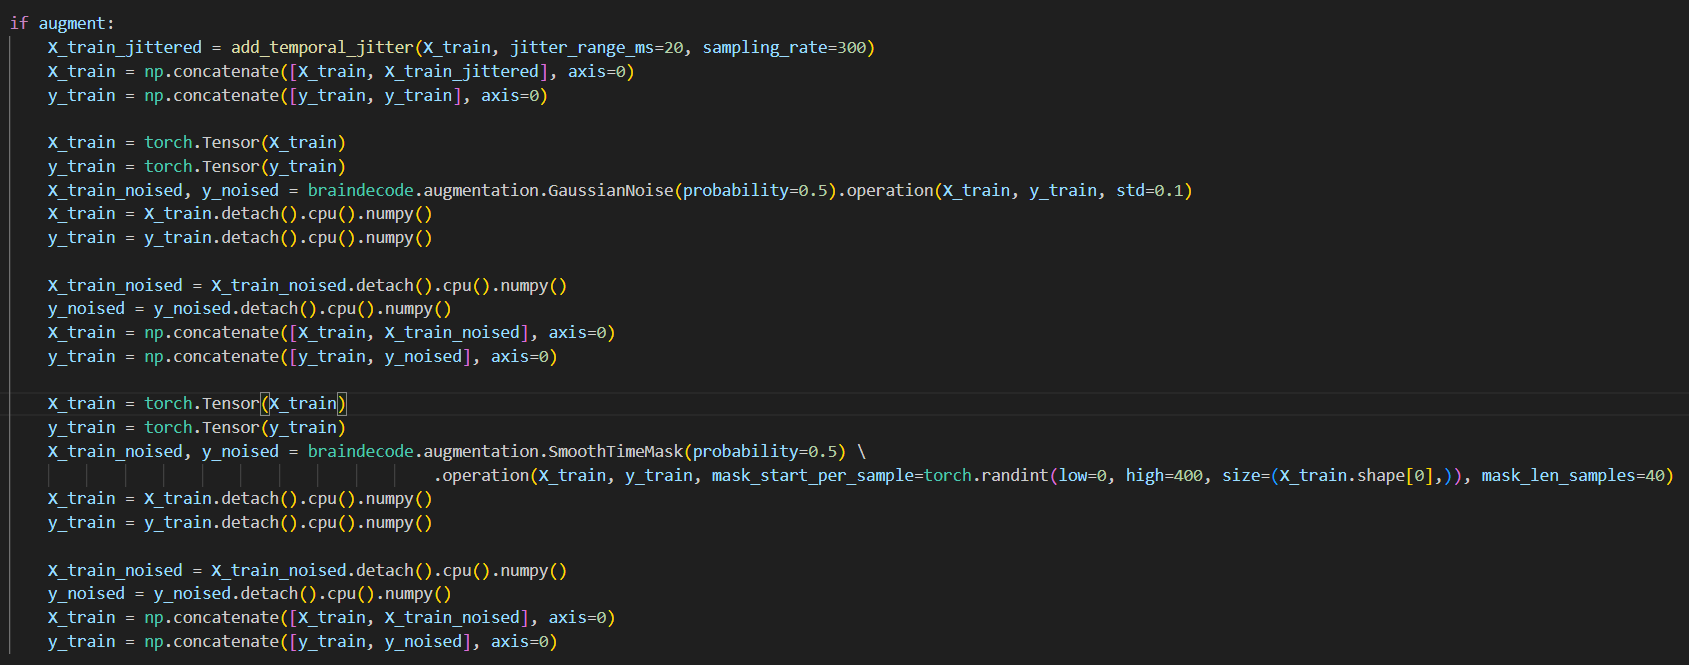
\includegraphics[width=1\linewidth]{images/augmentari.png}
    \caption{Augmentările datelor}
    \label{fig:augmentari}
\end{figure}

\begin{figure}
    \centering
    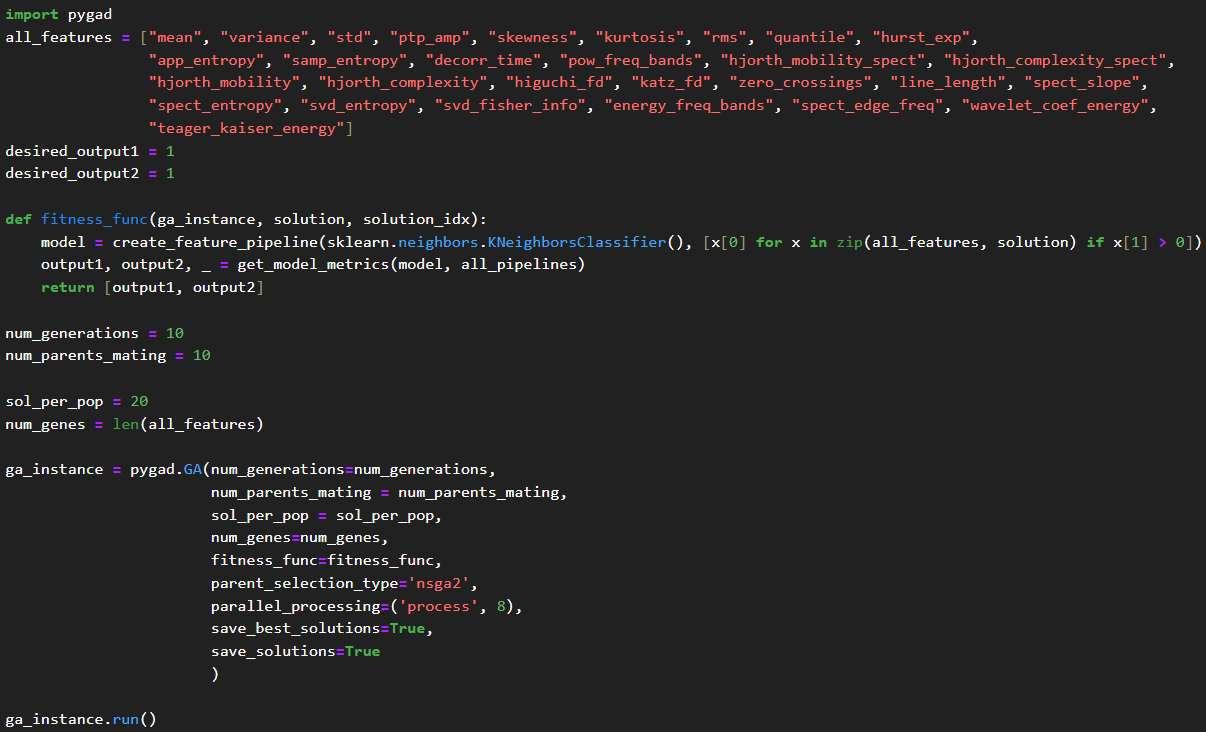
\includegraphics[width=1\linewidth]{pygad.png}
    \caption{Configurația librăriei pentru algoritmi genetici}
    \label{fig:pygad_configuration}
\end{figure}